\chapter{Data}
This chapter introduces the data used in the analysis and discuss how the data is processed and features are engineered. 

We use the Freddie Mac Single Familiy Loan-Level Dataset for the analysis, which they made available to the public at the direction of its regulators the Federal Housing Finance Agency (FHFA), in an attempt to increase data transparency \cite[p. 3]{Freddie_mac_guide}. The datset spans from the first quarter of 1999 to the third quarter of 2018 at the time of writing, however it should be noted that the dataset is a living dataset, in the sence that it is being updated at additional information could be added. We downloaded the data at the first february 2020, any changes that may occur after this date will not be taken into consideration. 

The dataset contains approximately 23 million  fully amortising 15, 20 and 20 year fixed-rate mortgages which together have over 2 billion monthly performance updates. The data is divided into two csv files each quarter one containing the Origination data and another containing the monthly Performance updates. The origination data contains static information given at the origination of the loan while the Performance updates include payment activity for each month. The payment activity variable (delq\_sts) is used to derive the target variable of the analysis. All the original features of the two datasets are available in Appendix \ref{app:Freddie_mac} Table \vref{tab:FM_origination_features} for the origination features and Table \vref{tab:FM_performance_features}. The features we choose to include in the analysis is listed in Appendix \ref{app:Freddie_mac} Table \vref{tab:included_features}.

The vast amount of data makes the data preprocessing as well as estimation of the models and simply plotting the data a challenge using a regular laptop, which is at our disposal. One solution towards this problem, is to run the analysis on a sample of the full dataset, however since we are using techniques which perform better the more data there are available to them, we choose another approach. The approach is to create a virtual machine on \href{https://cloud.google.com/}{Google Cloud}, which offers \$300 free usage for first time private users. Thus, on Google Cloud we configure a virtual machine with 1 CPU, and 60GB of memory and 150GB HDD, which should be enough. Then we install Ubuntu 18.04, R version 3.6.2 and Rstudio Server, which by typing in the external ip-adress and port 8787, we are able to work in Rstudio as we are used to on our laptop, the only difference is that everything is done on Googles servers and not on our own laptop. However, since the amount of data is so extreme, the data preprocessing still takes approximately 10 hours.

\begin{comment}
We are aware that factors outside this dataset such as unemployment rate per state GDP growth rate per state etc., could help explaining weather costumers default or not, however since the focus of this thesis is on explaining deep models rather than increase predictability we will not include these factors.  
\end{comment}


\section{Default Definition}
The dependent variable in this analysis is whether or not a costumer pays back his or hers mortgage if a costumer does not pay back the loan we put the costumer in the class >>Default<<

\begin{flalign}
\text{Default} & = \begin{cases} 
            1, \qquad \text{if mortgage is repayed } \\
            0, \qquad \text{if mortgage is not repayed}
            \end{cases}
\end{flalign}



\section{Data Cleaning}

\section{Data Exploration}
\begin{figure}
    \centering
    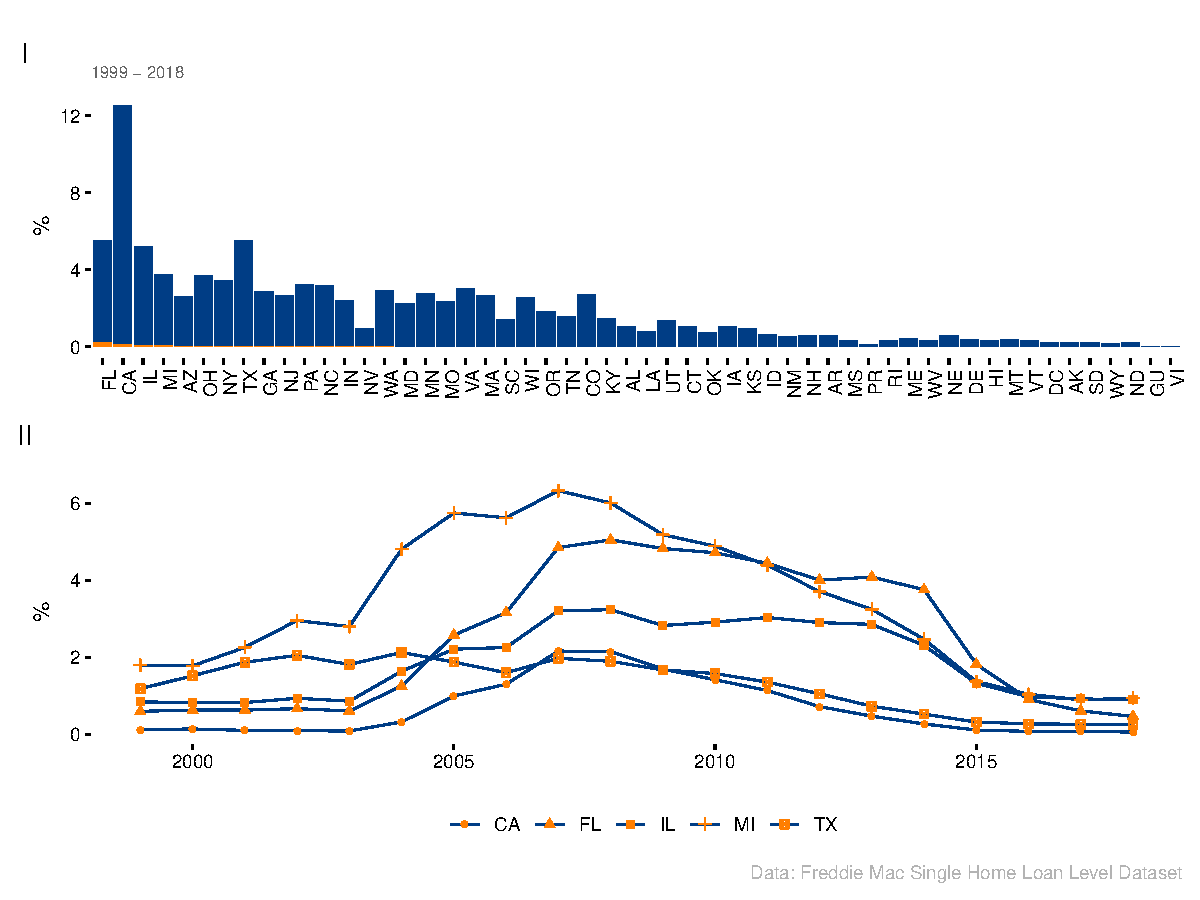
\includegraphics[width = \textwidth]{Figures/pw_3.pdf}
    \caption{Caption}
    \label{fig:my_label}
\end{figure}
        
\section{Data Processing}
    
        \subsection{Implementation}
        
        \subsection{Loading}
        
        \subsection{Manipulation}
        
        \subsection{Model Preparation}
        
    \section{Formal Description}
    
